\documentclass[11pt,a4paper]{article}

% ── Packages (only those available on this installation) ──────────────────────
\usepackage[margin=2.5cm]{geometry}
\usepackage{amsmath,amssymb}
\usepackage{graphicx}
\usepackage{booktabs}
\usepackage{longtable}
\usepackage{array}
\usepackage{xcolor}
\usepackage{hyperref}
\usepackage{caption}
\usepackage{subcaption}
\usepackage{enumitem}
\usepackage{microtype}
\usepackage{listings}
\usepackage{float}
\usepackage{placeins}
\IfFileExists{todonotes.sty}{\usepackage{todonotes}}{\newcommand{\todo}[2][]{}}

% ── Figure path ───────────────────────────────────────────────────────────────
\graphicspath{{figures/}}

% ── Hyperref setup ────────────────────────────────────────────────────────────
\hypersetup{
  colorlinks = true,
  linkcolor  = blue!70!black,
  citecolor  = green!50!black,
  urlcolor   = blue!70!black,
}

% ── Custom commands ───────────────────────────────────────────────────────────
\newcommand{\numu}{$\nu_\mu$}
\newcommand{\numubar}{$\bar{\nu}_\mu$}
\newcommand{\ccpip}{$\mathrm{CC}\pi^{\pm}$}
\newcommand{\pmu}{$p_\mu$}
\newcommand{\ppi}{$p_\pi$}
\newcommand{\costhmu}{$\cos\theta_\mu$}
\newcommand{\costhpi}{$\cos\theta_\pi$}
\newcommand{\thmupi}{$\theta_{\mu\pi}$}
\newcommand{\uboone}{MicroBooNE}
\newcommand{\GeVc}{\,\text{GeV}\!/c}
\newcommand{\pot}{\,\text{POT}}
\newcommand{\cm}{\,\text{cm}}

% inline math shorthand so they work inside math mode too
\newcommand{\pmuM}{p_\mu}
\newcommand{\ppiM}{p_\pi}
\newcommand{\cthmuM}{\cos\theta_\mu}
\newcommand{\cthpiM}{\cos\theta_\pi}
\newcommand{\thmupM}{\theta_{\mu\pi}}

% ── Listings (C++ snippets) ───────────────────────────────────────────────────
\lstset{
  language=C++,
  basicstyle=\ttfamily\small,
  keywordstyle=\bfseries\color{blue!70!black},
  commentstyle=\itshape\color{gray},
  backgroundcolor=\color{gray!10},
  frame=single,
  framerule=0.4pt,
  numbers=none,
  breaklines=true,
}

% ── Table column helpers ──────────────────────────────────────────────────────
\newcolumntype{C}[1]{>{\centering\arraybackslash}p{#1}}
\newcolumntype{R}[1]{>{\raggedleft\arraybackslash}p{#1}}
\newcolumntype{L}[1]{>{\raggedright\arraybackslash}p{#1}}

% Let TeX stretch spacing on hard-to-break lines (long \texttt paths/code) to keep
% text out of the margin.
\emergencystretch=3em

% ─────────────────────────────────────────────────────────────────────────────


% ---- cross-document references to the technical supplement ----
\usepackage{xr}
\externaldocument{analysis_note}
\externaldocument[S-]{technical_supplement}
\newcommand{\suppref}[2]{#1~\ref{S-#2} of the technical supplement}
\externaldocument[CR-]{cr_data_note}
\externaldocument[AR-]{approval_request}
\externaldocument[P-]{proton_tagged_note}
\newcommand{\ptref}[2]{#1~\ref{P-#2} of the proton-tagged note}
\newcommand{\noteref}[2]{#1~\ref{#2} of the analysis note}
\newcommand{\crref}[2]{#1~\ref{CR-#2} of the control-sample note}
\usepackage{tikz}
\usetikzlibrary{arrows.meta,positioning}
% Every result figure shows fake data. The stamp is drawn over the graphic by LaTeX so it cannot be
% dropped by regenerating the figure, and so black points are never mistaken for beam-on data.
\newcommand{\blindfig}[2][\textwidth]{%
  \begin{tikzpicture}
    \node[inner sep=0pt] (img) {\includegraphics[width=#1]{#2}};
    \node[anchor=north east, fill=red!12, draw=red!60!black, rounded corners=1pt, inner sep=2pt,
          font=\scriptsize\bfseries\sffamily, text=red!60!black] at ([xshift=-2pt,yshift=-2pt]img.north east)
          {BLINDED: CV PSEUDO-DATA};
  \end{tikzpicture}}


\input{glyphtounicode}
\pdfgentounicode=1

\begin{document}
\begin{center}
{\LARGE\bfseries Beam-on control-region material held out of the analysis documents\par}
\vspace{0.4cm}{\large 2026-09-27\par}
\end{center}

The analysis note, the proton-tagged note and the technical supplement are written as they stand
before the control regions are compared with beam-on data. Every passage that used beam-on data was
removed from them on 2026-09-27 and is kept below, verbatim, for merging back once the comparison is
presented. Each entry gives the document and place it came from, the original LaTeX source and the source
that replaced it (the whole subsection is also typeset). The label \texttt{sec:cr\_outcome} and the figure \texttt{fig:cr\_data} now
exist only here; the analysis note has \texttt{sec:cr\_procedure} in their place. The detailed
comparison itself is in the control-sample note (\texttt{cr\_data\_note.tex}). Since 2026-09-28 the
prerequisites that the passages cite as \texttt{sec:unblinding} are in the approval request
(\texttt{approval\_request.tex}), and the replacement passages quoted below have been revised since.

\section{analysis\_note.tex: abstract}
\paragraph{Original source.}
\begin{lstlisting}[language={[LaTeX]TeX},basicstyle=\ttfamily\footnotesize,columns=fullflexible]
    The signal region is blind, and all results are extracted from Poisson
    fluctuations of the central-value simulation. The four background control regions have been
    compared with beam-on data: they require no correction of the background model, and the data lie
    $12$--$20\%$ above the prediction, within its flux and cross-section uncertainties, in every run
    period except FHC Run~1, whose $13\%$ offset from the other periods is not yet explained. The
    extraction
\end{lstlisting}
\paragraph{Replaced by.}
\begin{lstlisting}[language={[LaTeX]TeX},basicstyle=\ttfamily\footnotesize,columns=fullflexible]
    The signal region is blind, and all results are extracted from Poisson
    fluctuations of the central-value simulation. Four background control regions, disjoint from the
    signal region, are defined for a comparison with beam-on data under a frozen procedure, and the
    request to open them is part of this note. The
    extraction
\end{lstlisting}

\section{analysis\_note.tex: Sec. 1.1 (measurement overview), blindness paragraph}
\paragraph{Original source.}
\begin{lstlisting}[language={[LaTeX]TeX},basicstyle=\ttfamily\footnotesize,columns=fullflexible]
The four background control regions are disjoint from the
signal region and have been compared with beam-on data (\S\ref{sec:cr_outcome}).
\end{lstlisting}
\paragraph{Replaced by.}
\begin{lstlisting}[language={[LaTeX]TeX},basicstyle=\ttfamily\footnotesize,columns=fullflexible]
The four background control regions are disjoint from the
signal region and are to be compared with beam-on data under the frozen procedure of
\S\ref{sec:cr}.
\end{lstlisting}

\section{analysis\_note.tex: Sec. 1.1, approval paragraph}
\paragraph{Original source.}
\begin{lstlisting}[language={[LaTeX]TeX},basicstyle=\ttfamily\footnotesize,columns=fullflexible]
approval. Opening the signal region further requires the items listed in
\S\ref{sec:unblinding}, among them the confirmation of the absolute flux normalisation and an
understanding of the FHC Run-1 offset seen in the control regions.
\end{lstlisting}
\paragraph{Replaced by.}
\begin{lstlisting}[language={[LaTeX]TeX},basicstyle=\ttfamily\footnotesize,columns=fullflexible]
approval, together with the request to compare the control regions with beam-on data. Opening the
signal region further requires the items listed in \S\ref{sec:unblinding}, among them the
confirmation of the absolute flux normalisation.
\end{lstlisting}

\section{analysis\_note.tex: Sec. 1.1, pointer paragraph}
\paragraph{Original source.}
\begin{lstlisting}[language={[LaTeX]TeX},basicstyle=\ttfamily\footnotesize,columns=fullflexible]
cross-checks behind the choices described here are collected in the technical supplement, and the
comparison of the control regions with beam-on data in the control-sample note. The
\end{lstlisting}
\paragraph{Replaced by.}
\begin{lstlisting}[language={[LaTeX]TeX},basicstyle=\ttfamily\footnotesize,columns=fullflexible]
cross-checks behind the choices described here are collected in the technical supplement. The
\end{lstlisting}

\section{analysis\_note.tex: Sec. 9.1 (region definitions), pseudo-data test}
\paragraph{Original source.}
\begin{lstlisting}[language={[LaTeX]TeX},basicstyle=\ttfamily\footnotesize,columns=fullflexible]
Before the comparison with beam-on data, the region definitions and the per-run normalisation were
tested on pseudo-data
\end{lstlisting}
\paragraph{Replaced by.}
\begin{lstlisting}[language={[LaTeX]TeX},basicstyle=\ttfamily\footnotesize,columns=fullflexible]
The region definitions and the per-run normalisation are tested on pseudo-data
\end{lstlisting}

\section{analysis\_note.tex: Sec. 9.1, caption of tab:sidebands}
\paragraph{Original source.}
\begin{lstlisting}[language={[LaTeX]TeX},basicstyle=\ttfamily\footnotesize,columns=fullflexible]
checks the region definitions and the per-run normalisation; the background model is tested with
    beam-on data (\S\ref{sec:cr_outcome}).}
\end{lstlisting}
\paragraph{Replaced by.}
\begin{lstlisting}[language={[LaTeX]TeX},basicstyle=\ttfamily\footnotesize,columns=fullflexible]
checks the region definitions and the per-run normalisation; the background model is to be
    tested with beam-on data (\S\ref{sec:cr_procedure}).}
\end{lstlisting}

\section{analysis\_note.tex: Sec. 9.2, the whole subsection "Comparison with beam-on data" (label sec:cr\_outcome) with fig:cr\_data}
\paragraph{Original source.}
\begin{lstlisting}[language={[LaTeX]TeX},basicstyle=\ttfamily\footnotesize,columns=fullflexible]
\subsection{Comparison with beam-on data}
\label{sec:cr_outcome}

The four regions have been compared with beam-on data at reconstruction level
(Fig.~\ref{fig:cr_data}), under a procedure fixed beforehand: frozen region definitions, a
pre-agreed test statistic and the conditions under which a correction may be applied
(\suppref{Sec.}{sec:request}). No beam-on sample of Run~2 exists, and Run~2 is removed from both data
and prediction in this comparison.

\begin{itemize}\itemsep3pt
  \item \textbf{Global test.} The frozen global test passes, $\chi^2=8.1/8$ ($p=0.42$).
  \item \textbf{No class-specific correction.} A joint FHC$+$RHC fit of the background-class
    normalisations gives the dominant CC$0\pi$ class at $0.949\pm0.190$ over all run periods
    ($0.984\pm0.191$ without FHC Run~1), consistent with unity (\crref{Sec.}{sec:jointfit}). The
    nominal background prediction is kept. The fit uses the CC$0\pi$, $\pi^0$ and cosmic regions; the
    multi-$\pi$ region, which shares $47$ FHC and $68$ RHC events with the $\pi^0$ region, is
    diagnostic and not in the fit, so the overlap does not enter the fit covariance.
  \item \textbf{Common excess.} The neutrino-dominated regions lie $12$--$20\%$ above the prediction,
    within the correlated flux and cross-section uncertainties. The excess does not follow the
    signal content of a region: tightening each region to reduce its signal (the CC$0\pi$ region from
    $8.6\%$ to $2.2\%$ signal while keeping $58\%$ of its events) leaves the data-to-prediction ratio
    unchanged, $1.12$ to $1.13$ (\crref{Sec.}{sec:farsb}), and the cosmic region approaches unity as
    its beam-off share increases. The excess therefore lies in the neutrino simulation and is not
    signal in the control regions.
  \item \textbf{FHC Run~1.} Period by period, the data lie $12$--$25\%$ above the prediction in every
    run period except FHC Run~1, which is consistent with unity (\crref{Table}{tab:perperiod_corrected}).
    A free normalisation factor on FHC Run~1 fits $0.869\pm0.022$ and improves the per-period fit by
    $\Delta\chi^2=37$, while a free factor on any other period gains at most $15$. The common excess
    of the other periods is covered by the correlated uncertainties; a $13\%$ offset of one period
    relative to the others is not. The cosmic region, dominated by beam-off events, is at
    $0.95\pm0.17$ in Run~1, so the Run-1 trigger count is not obviously wrong; the POT bookkeeping,
    the completeness of the Run-1 beam-on sample with respect to its run list and the normalisation of
    the Run-1 overlay remain to be checked (\S\ref{sec:unblinding}). The same comparison fixes the
    Run-1 exposure assignment: normalised to the open-trigger bookkeeping ($3.283\times10^{20}$~POT and
    $9\,846\,635$ triggers), FHC Run~1 lies at $0.60$--$0.72$ in the CC$0\pi$, $\pi^0$ and cosmic
    regions, with a fitted exposure factor of $0.520\pm0.020$, whereas the non-open-trigger values used
    here ($2.192\times10^{20}$~POT and $5\,748\,692$ triggers) give $0.95$--$1.10$ in the same regions.
  \item \textbf{Muon-momentum shape.} In two dimensions ($\cos\theta_\mu\times p_\mu$) the residual is
    organised in $p_\mu$: the data over the prediction are $1.16$--$1.82$ in the $0.35$--$0.75$~GeV/$c$
    bins, $1.05$--$1.40$ below and mostly $0.8$--$1.1$ above, in every angular bin, in both modes and in
    regions of different composition. Normalisation parameters do not remove it. It points to the
    muon momentum rather than to a background class, remains open, and two-dimensional
    normalisation fits are not quoted while it stands (\crref{Sec.}{sec:jointfit}).
\end{itemize}

A normalisation fit propagated under the frozen rules cannot reduce the uncertainty of the
measurement. Conditioning the prediction on the control-region totals could, through the flux and
detector correlations: on an Asimov dataset it reduces the uncertainty of the one-bin total from
$35.8\%$ to $11.3\%$ (\crref{Sec.}{sec:jointfit}). Adopting such a constraint would change the role
of the control regions and requires a collaboration decision.

\begin{figure}[H]
  \centering
  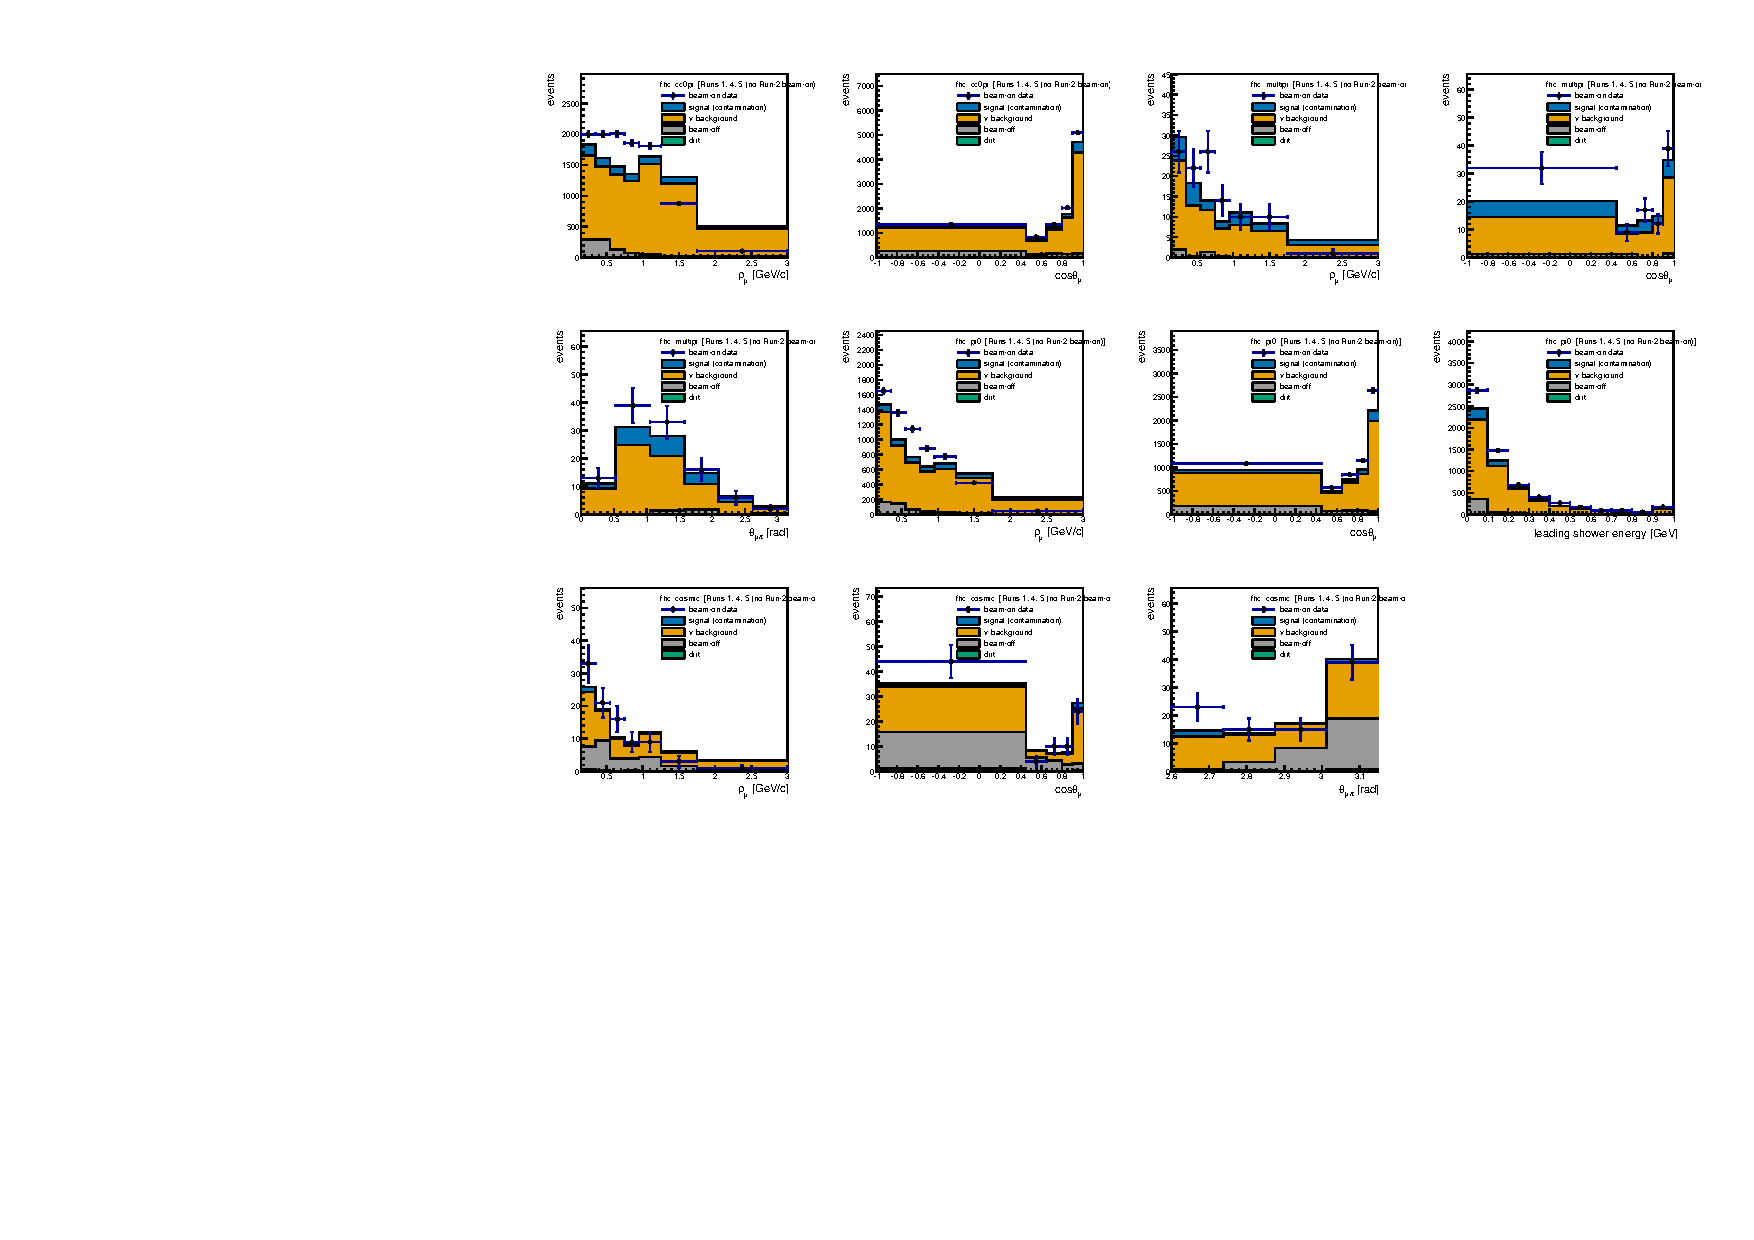
\includegraphics[width=0.96\textwidth]{sideband_data_fhc}\\[4pt]
  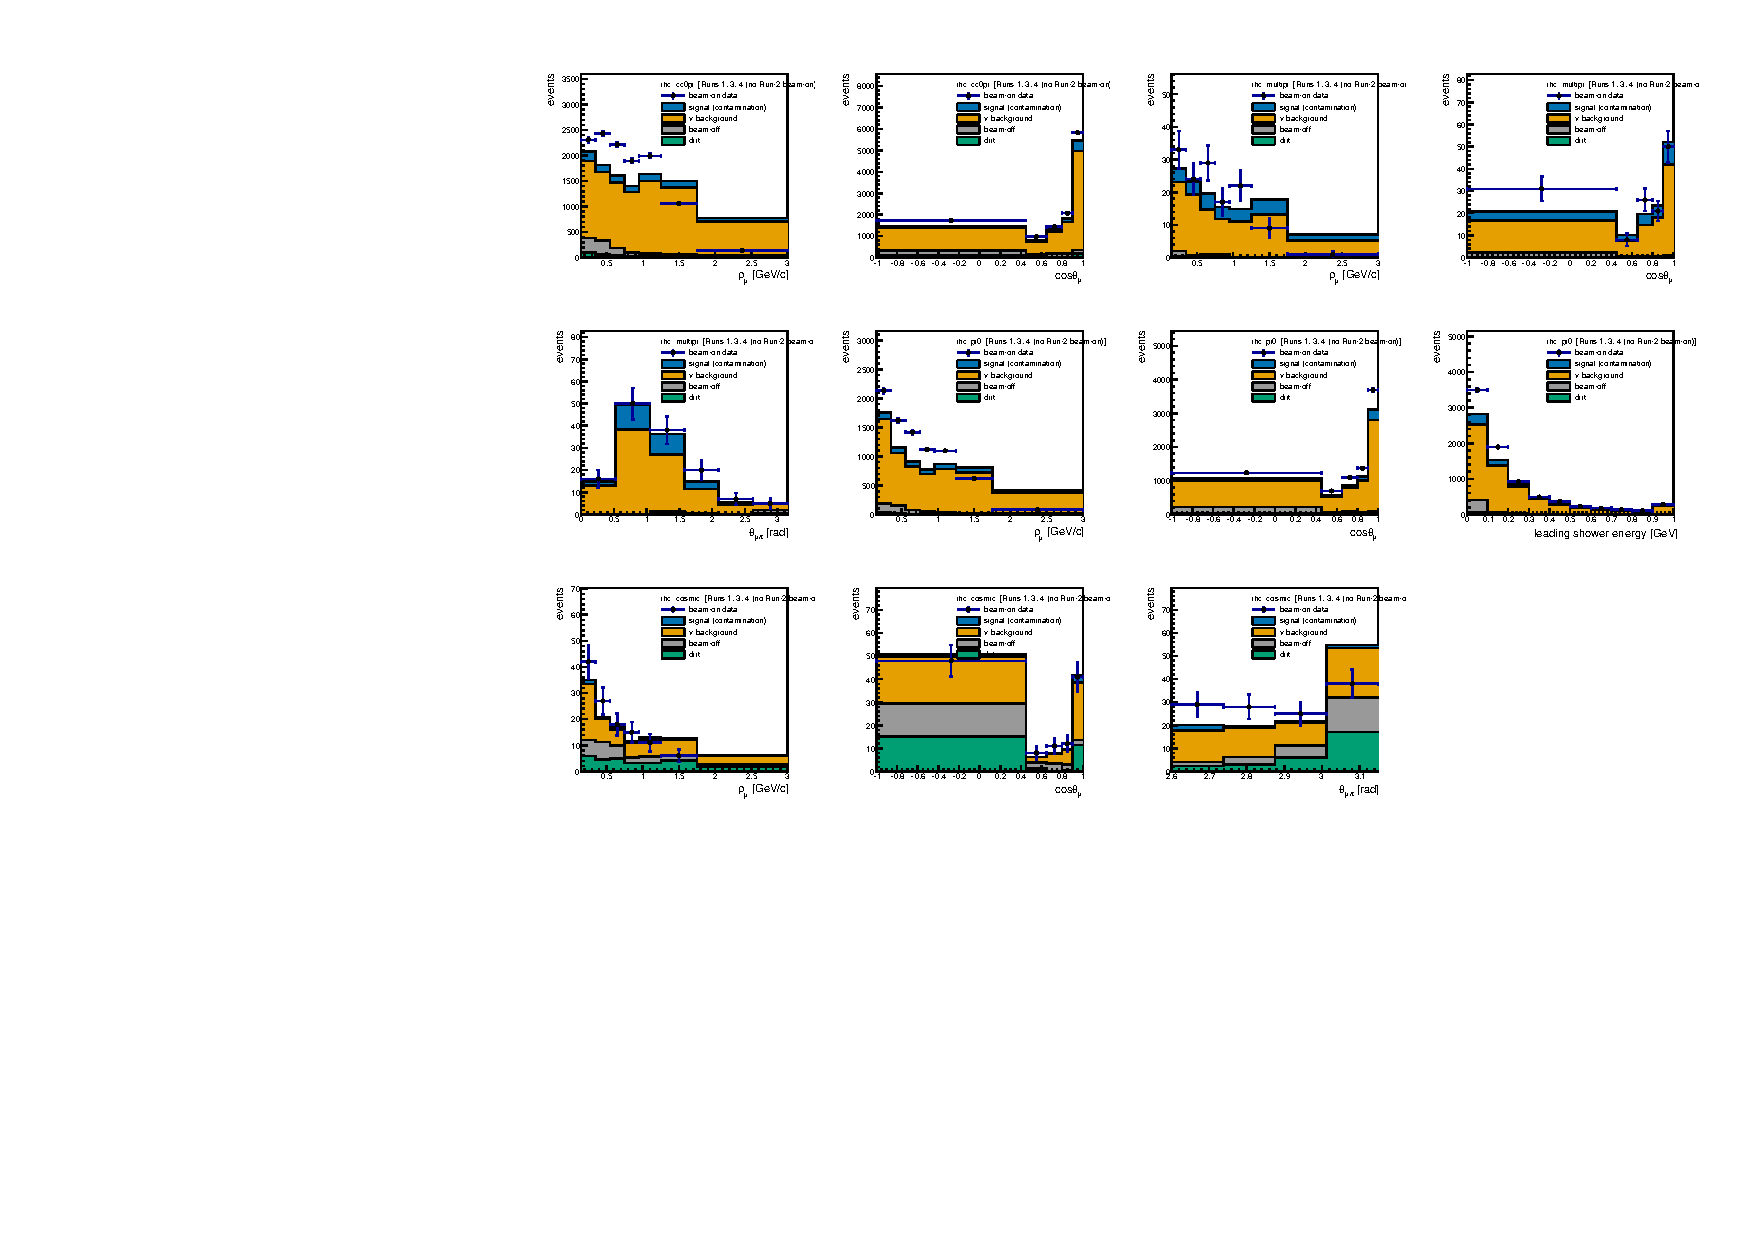
\includegraphics[width=0.96\textwidth]{sideband_data_rhc}
  \caption{The control regions with beam-on data: FHC (top) and RHC (bottom), data compared with the
    neutrino simulation $+$ beam-off $+$ dirt prediction in each region, normalised to the exposure of
    the run periods with beam-on data (Run~2 has none). The ratios per run period, the fitted
    normalisations and their correlations are in the control-sample note.}
  \label{fig:cr_data}
\end{figure}
\end{lstlisting}
\paragraph{Replaced by.}
\begin{lstlisting}[language={[LaTeX]TeX},basicstyle=\ttfamily\footnotesize,columns=fullflexible]
\subsection{Comparison with beam-on data}
\label{sec:cr_procedure}

The four regions are to be compared with beam-on data at reconstruction level under a procedure
fixed before the data are examined: frozen region definitions, a pre-agreed test statistic and the
conditions under which a correction to the background model may be applied
(\suppref{Sec.}{sec:request} and \suppref{Sec.}{sec:cr_protocol}). No beam-on sample of Run~2 exists,
so Run~2 is removed from both data and prediction in this comparison. The pseudo-data studies of
\S\ref{sec:sidebands} and the full-stack test of \suppref{Sec.}{sec:cr_fullstack} exercise the same
path with simulated data.

A normalisation fit propagated under the frozen rules cannot reduce the uncertainty of the
measurement. Conditioning the prediction on the control-region totals could, through the flux and
detector correlations: on an Asimov dataset it reduces the uncertainty of the one-bin total from
$35.8\%$ to $11.3\%$. Adopting such a constraint would change the role of the control regions and
requires a collaboration decision.
\end{lstlisting}
\paragraph{Original, typeset.}
\begingroup
\subsection{Comparison with beam-on data}
\label{sec:cr_outcome}

The four regions have been compared with beam-on data at reconstruction level
(Fig.~\ref{fig:cr_data}), under a procedure fixed beforehand: frozen region definitions, a
pre-agreed test statistic and the conditions under which a correction may be applied
(\suppref{Sec.}{sec:request}). No beam-on sample of Run~2 exists, and Run~2 is removed from both data
and prediction in this comparison.

\begin{itemize}\itemsep3pt
  \item \textbf{Global test.} The frozen global test passes, $\chi^2=8.1/8$ ($p=0.42$).
  \item \textbf{No class-specific correction.} A joint FHC$+$RHC fit of the background-class
    normalisations gives the dominant CC$0\pi$ class at $0.949\pm0.190$ over all run periods
    ($0.984\pm0.191$ without FHC Run~1), consistent with unity (\crref{Sec.}{sec:jointfit}). The
    nominal background prediction is kept. The fit uses the CC$0\pi$, $\pi^0$ and cosmic regions; the
    multi-$\pi$ region, which shares $47$ FHC and $68$ RHC events with the $\pi^0$ region, is
    diagnostic and not in the fit, so the overlap does not enter the fit covariance.
  \item \textbf{Common excess.} The neutrino-dominated regions lie $12$--$20\%$ above the prediction,
    within the correlated flux and cross-section uncertainties. The excess does not follow the
    signal content of a region: tightening each region to reduce its signal (the CC$0\pi$ region from
    $8.6\%$ to $2.2\%$ signal while keeping $58\%$ of its events) leaves the data-to-prediction ratio
    unchanged, $1.12$ to $1.13$ (\crref{Sec.}{sec:farsb}), and the cosmic region approaches unity as
    its beam-off share increases. The excess therefore lies in the neutrino simulation and is not
    signal in the control regions.
  \item \textbf{FHC Run~1.} Period by period, the data lie $12$--$25\%$ above the prediction in every
    run period except FHC Run~1, which is consistent with unity (\crref{Table}{tab:perperiod_corrected}).
    A free normalisation factor on FHC Run~1 fits $0.869\pm0.022$ and improves the per-period fit by
    $\Delta\chi^2=37$, while a free factor on any other period gains at most $15$. The common excess
    of the other periods is covered by the correlated uncertainties; a $13\%$ offset of one period
    relative to the others is not. The cosmic region, dominated by beam-off events, is at
    $0.95\pm0.17$ in Run~1, so the Run-1 trigger count is not obviously wrong; the POT bookkeeping,
    the completeness of the Run-1 beam-on sample with respect to its run list and the normalisation of
    the Run-1 overlay remain to be checked (Sec.~\ref{AR-sec:ar_prereq} of the approval request). The same comparison fixes the
    Run-1 exposure assignment: normalised to the open-trigger bookkeeping ($3.283\times10^{20}$~POT and
    $9\,846\,635$ triggers), FHC Run~1 lies at $0.60$--$0.72$ in the CC$0\pi$, $\pi^0$ and cosmic
    regions, with a fitted exposure factor of $0.520\pm0.020$, whereas the non-open-trigger values used
    here ($2.192\times10^{20}$~POT and $5\,748\,692$ triggers) give $0.95$--$1.10$ in the same regions.
  \item \textbf{Muon-momentum shape.} In two dimensions ($\cos\theta_\mu\times p_\mu$) the residual is
    organised in $p_\mu$: the data over the prediction are $1.16$--$1.82$ in the $0.35$--$0.75$~GeV/$c$
    bins, $1.05$--$1.40$ below and mostly $0.8$--$1.1$ above, in every angular bin, in both modes and in
    regions of different composition. Normalisation parameters do not remove it. It points to the
    muon momentum rather than to a background class, remains open, and two-dimensional
    normalisation fits are not quoted while it stands (\crref{Sec.}{sec:jointfit}).
\end{itemize}

A normalisation fit propagated under the frozen rules cannot reduce the uncertainty of the
measurement. Conditioning the prediction on the control-region totals could, through the flux and
detector correlations: on an Asimov dataset it reduces the uncertainty of the one-bin total from
$35.8\%$ to $11.3\%$ (\crref{Sec.}{sec:jointfit}). Adopting such a constraint would change the role
of the control regions and requires a collaboration decision.

\begin{figure}[H]
  \centering
  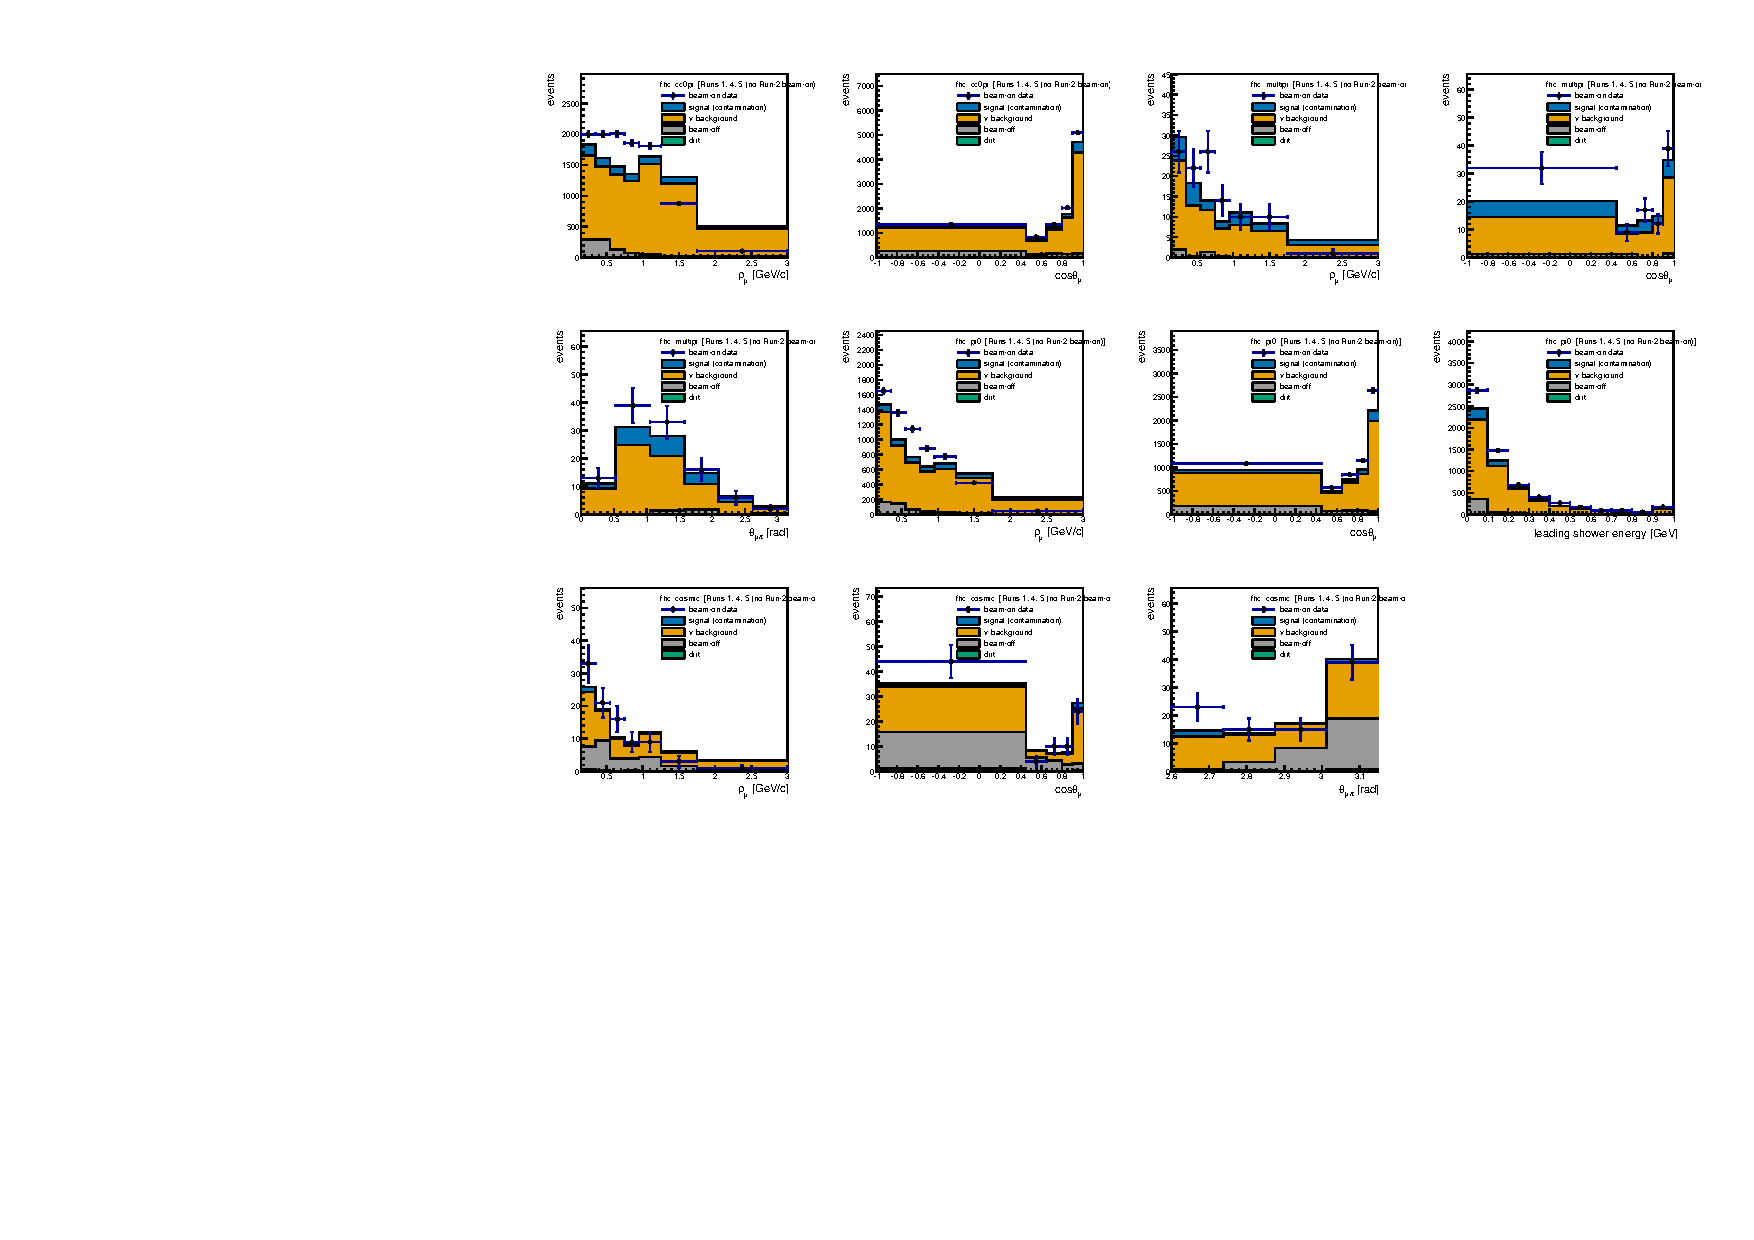
\includegraphics[width=0.96\textwidth]{sideband_data_fhc}\\[4pt]
  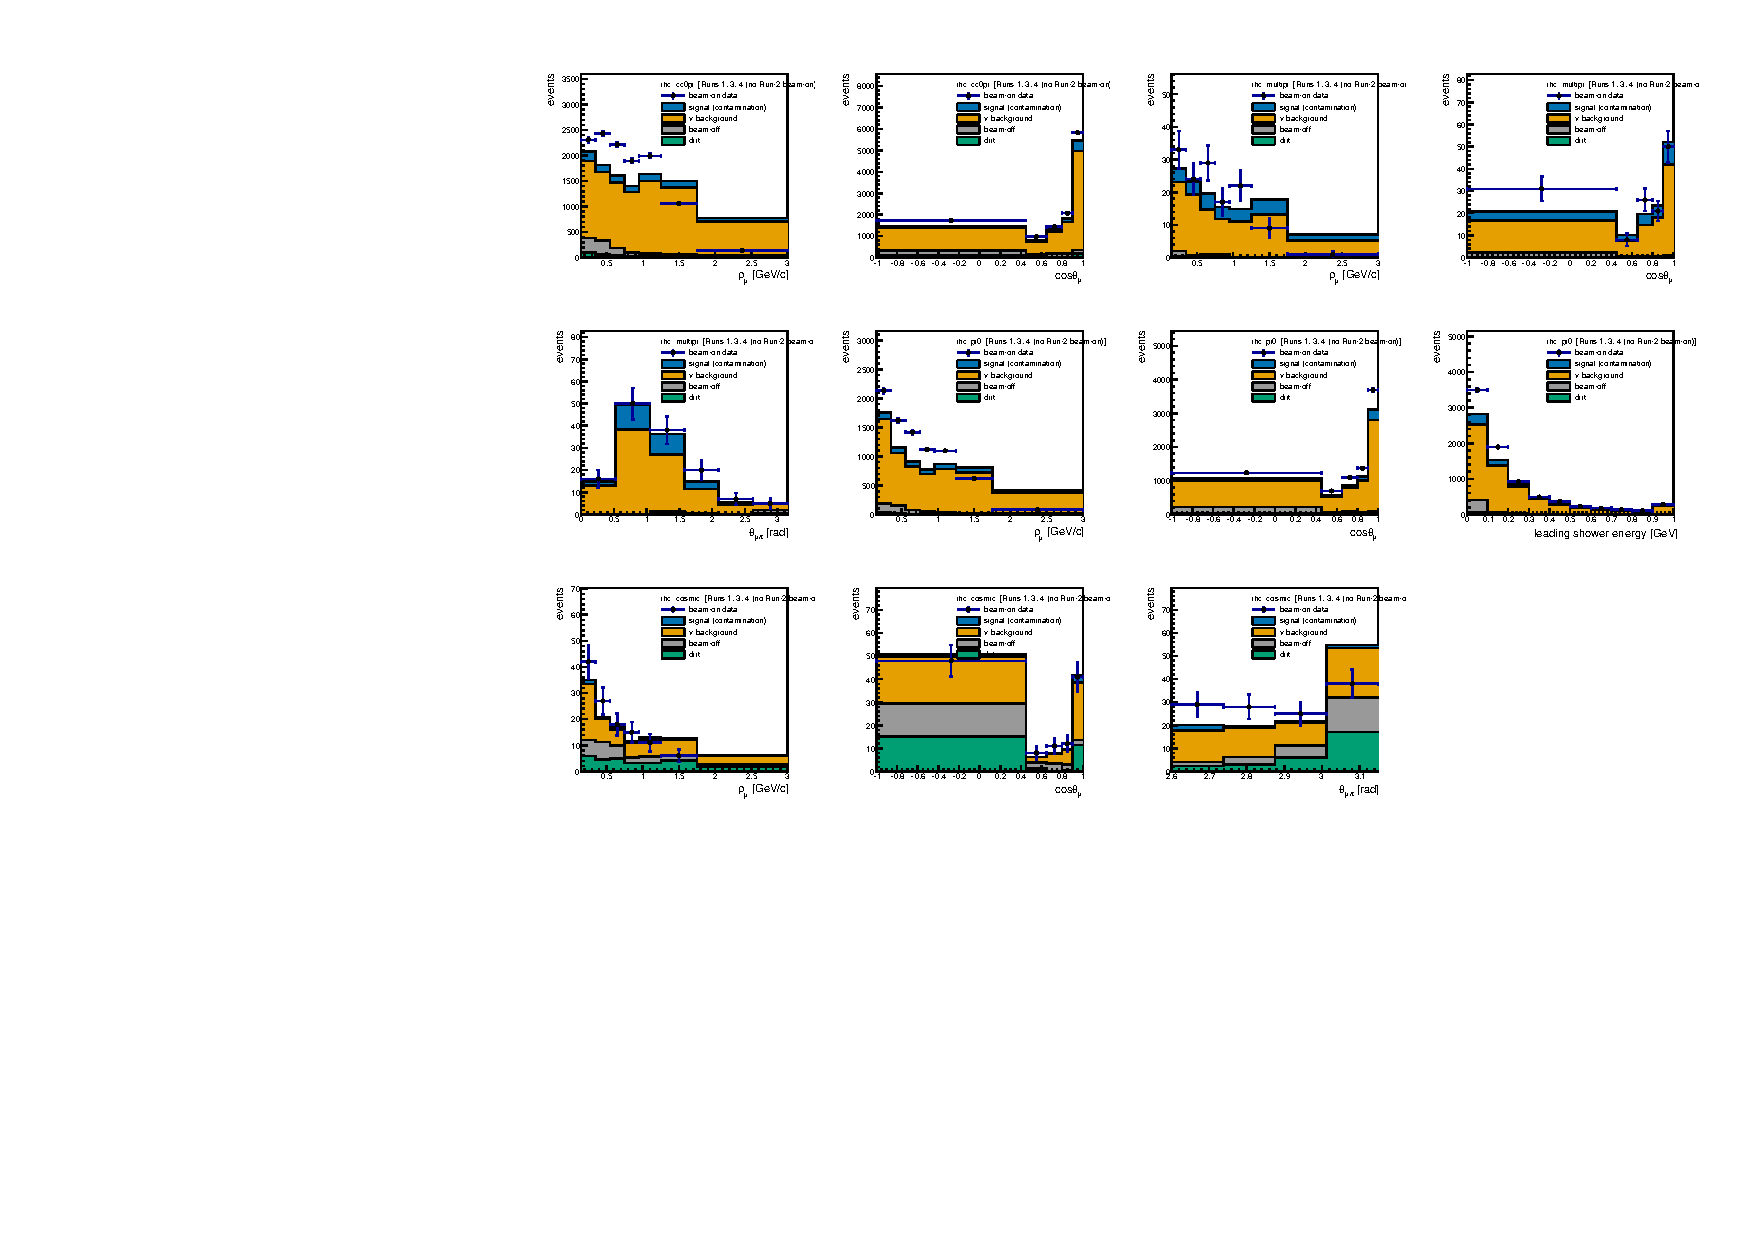
\includegraphics[width=0.96\textwidth]{sideband_data_rhc}
  \caption{The control regions with beam-on data: FHC (top) and RHC (bottom), data compared with the
    neutrino simulation $+$ beam-off $+$ dirt prediction in each region, normalised to the exposure of
    the run periods with beam-on data (Run~2 has none). The ratios per run period, the fitted
    normalisations and their correlations are in the control-sample note.}
  \label{fig:cr_data}
\end{figure}


\endgroup

\section{analysis\_note.tex: Sec. 9.3 (validation of the background fit), first sentence}
\paragraph{Original source.}
\begin{lstlisting}[language={[LaTeX]TeX},basicstyle=\ttfamily\footnotesize,columns=fullflexible]
The background fit was validated on simulation before it was applied to data: toy ensembles give
\end{lstlisting}
\paragraph{Replaced by.}
\begin{lstlisting}[language={[LaTeX]TeX},basicstyle=\ttfamily\footnotesize,columns=fullflexible]
The background fit is validated on simulation: toy ensembles give
\end{lstlisting}

\section{analysis\_note.tex: Sec. 14 (limitations), blind signal region}
\paragraph{Original source.}
\begin{lstlisting}[language={[LaTeX]TeX},basicstyle=\ttfamily\footnotesize,columns=fullflexible]
provides the fake data and the background estimate. It has been tested at reconstruction level in
the four control regions (\S\ref{sec:cr_outcome}), which require no correction; the offset of FHC
Run~1 relative to the other run periods is not yet explained.
\end{lstlisting}
\paragraph{Replaced by.}
\begin{lstlisting}[language={[LaTeX]TeX},basicstyle=\ttfamily\footnotesize,columns=fullflexible]
provides the fake data and the background estimate. The four control regions are defined to test it
at reconstruction level with beam-on data (\S\ref{sec:cr}).
\end{lstlisting}

\section{analysis\_note.tex: Sec. 14.1 (requirements for unblinding), list item 2}
\paragraph{Original source.}
\begin{lstlisting}[language={[LaTeX]TeX},basicstyle=\ttfamily\footnotesize,columns=fullflexible]
  \item an understanding of the $13\%$ offset of FHC Run~1 relative to the other run periods in the
    control regions: its exposure bookkeeping, the completeness of its beam-on sample and the
    normalisation of its overlay (\S\ref{sec:cr_outcome});
\end{lstlisting}
\paragraph{Replaced by.}
\begin{lstlisting}[language={[LaTeX]TeX},basicstyle=\ttfamily\footnotesize,columns=fullflexible]
  \item the comparison of the control regions with beam-on data under the frozen procedure, and the
    treatment of any discrepancy under that procedure (\S\ref{sec:cr_procedure});
\end{lstlisting}

\section{analysis\_note.tex: Sec. 14.1, closing paragraph}
\paragraph{Original source.}
\begin{lstlisting}[language={[LaTeX]TeX},basicstyle=\ttfamily\footnotesize,columns=fullflexible]
The control regions were compared with beam-on data under the frozen procedure of
\suppref{Sec.}{sec:cr_protocol}, and any correction to the background model follows that procedure.
No switch
\end{lstlisting}
\paragraph{Replaced by.}
\begin{lstlisting}[language={[LaTeX]TeX},basicstyle=\ttfamily\footnotesize,columns=fullflexible]
Any correction to the background model follows the frozen procedure of
\suppref{Sec.}{sec:cr_protocol}. No switch
\end{lstlisting}

\section{analysis\_note.tex: Sec. 15 (summary), background paragraph}
\paragraph{Original source.}
\begin{lstlisting}[language={[LaTeX]TeX},basicstyle=\ttfamily\footnotesize,columns=fullflexible]
\paragraph{Background.}
The four control regions, disjoint from the signal region, have been compared with beam-on data. The
global test passes ($\chi^2=8.1/8$), no class-specific correction of the background is supported,
and the data lie $12$--$20\%$ above the prediction, within the flux and cross-section uncertainties,
in every run period except FHC Run~1, whose offset of $13\%$ relative to the others is under
investigation.
\end{lstlisting}
\paragraph{Replaced by.}
\begin{lstlisting}[language={[LaTeX]TeX},basicstyle=\ttfamily\footnotesize,columns=fullflexible]
\paragraph{Background.}
The background, $41$--$42\%$ of the selected sample, is taken from the simulation and from beam-off
data. Four control regions, disjoint from the signal region, test the prediction; they have been
validated with pseudo-data and are to be compared with beam-on data under a frozen procedure.
\end{lstlisting}

\section{analysis\_note.tex: Sec. 15, limitations paragraph}
\paragraph{Original source.}
\begin{lstlisting}[language={[LaTeX]TeX},basicstyle=\ttfamily\footnotesize,columns=fullflexible]
normalisation must be confirmed, the FHC Run-1 offset understood and a closure test with an
independent generator made (\S\ref{sec:unblinding}).
\end{lstlisting}
\paragraph{Replaced by.}
\begin{lstlisting}[language={[LaTeX]TeX},basicstyle=\ttfamily\footnotesize,columns=fullflexible]
normalisation must be confirmed, the control regions compared with beam-on data and a closure test
with an independent generator made (\S\ref{sec:unblinding}).
\end{lstlisting}

\section{proton\_tagged\_note.tex: Sec. 2.1 (what the proton candidate is)}
\paragraph{Original source.}
\begin{lstlisting}[language={[LaTeX]TeX},basicstyle=\ttfamily\footnotesize,columns=fullflexible]
The multi-$\pi$ control region of the inclusive analysis, already compared with beam-on data,
receives
\end{lstlisting}
\paragraph{Replaced by.}
\begin{lstlisting}[language={[LaTeX]TeX},basicstyle=\ttfamily\footnotesize,columns=fullflexible]
The multi-$\pi$ control region of the inclusive analysis receives
\end{lstlisting}

\section{technical\_supplement.tex: Sec. "Control regions: the opening request and its sign-off" (sec:request), opening paragraph}
\paragraph{Original source.}
\begin{lstlisting}[language={[LaTeX]TeX},basicstyle=\ttfamily\footnotesize,columns=fullflexible]
The four reconstruction-level control regions of the inclusive $\mathrm{CC}\,1\mu1\pi Xp$
selection have been compared with beam-on data under the procedure of this section, with the
signal region blind. The frozen global test passes ($\chi^2=8.1/8$, $p=0.42$); the joint FHC$+$RHC
fit gives the CC$0\pi$ class at $0.949\pm0.190$ ($0.984\pm0.191$ without FHC Run~1), and no
class-specific correction is applied. Two items remain open: FHC Run~1 lies $13\%$ below the other
run periods (a free factor of $0.869\pm0.022$, $\Delta\chi^2=37$), and the two-dimensional
comparison shows a residual organised in $p_\mu$ (\noteref{Sec.}{sec:cr_outcome}). The request
under which the regions were opened, and the state of the analysis it refers to, are recorded
below; \noteref{Sec.}{sec:sidebands} gives the region definitions.
\end{lstlisting}
\paragraph{Replaced by.}
\begin{lstlisting}[language={[LaTeX]TeX},basicstyle=\ttfamily\footnotesize,columns=fullflexible]
The decision requested of the collaboration is permission to inspect beam-on data in four
reconstruction-level control regions of the inclusive $\mathrm{CC}\,1\mu1\pi Xp$ selection while
the signal region stays blind. \noteref{Sec.}{sec:sidebands} gives the region definitions; the
numbers are those of the frozen state identified in the box below.
\end{lstlisting}

\section{technical\_supplement.tex: Sec. consistency with the nu\_e measurement, POT accounting item}
\paragraph{Original source.}
\begin{lstlisting}[language={[LaTeX]TeX},basicstyle=\ttfamily\footnotesize,columns=fullflexible]
non-open-trigger dataset, $2.192\times10^{20}$~POT with $5\,748\,692$ triggers, confirmed
against the beam bookkeeping and, independently, by the control-region exposure test
(\noteref{Sec.}{sec:cr_outcome}); the total
\end{lstlisting}
\paragraph{Replaced by.}
\begin{lstlisting}[language={[LaTeX]TeX},basicstyle=\ttfamily\footnotesize,columns=fullflexible]
non-open-trigger dataset, $2.192\times10^{20}$~POT with $5\,748\,692$ triggers, confirmed
against the beam bookkeeping; the total
\end{lstlisting}

\section{technical\_supplement.tex: Sec. control-region machinery, full-stack pseudo-data test}
\paragraph{Original source.}
\begin{lstlisting}[language={[LaTeX]TeX},basicstyle=\ttfamily\footnotesize,columns=fullflexible]
beam modes, the frozen distributions exactly as they are drawn for the beam-on
comparison, with the same full-stack pseudo-data in place of the beam-on points.
\end{lstlisting}
\paragraph{Replaced by.}
\begin{lstlisting}[language={[LaTeX]TeX},basicstyle=\ttfamily\footnotesize,columns=fullflexible]
beam modes, the frozen distributions exactly as they will be drawn for the beam-on
comparison, with full-stack pseudo-data in place of the beam-on points.
\end{lstlisting}

\section{technical\_supplement.tex: Sec. control-region machinery, caption of the full-stack figures}
\paragraph{Original source.}
\begin{lstlisting}[language={[LaTeX]TeX},basicstyle=\ttfamily\footnotesize,columns=fullflexible]
The beam-on comparison uses
    these plots with the beam-on points in place of the pseudo-data;
\end{lstlisting}
\paragraph{Replaced by.}
\begin{lstlisting}[language={[LaTeX]TeX},basicstyle=\ttfamily\footnotesize,columns=fullflexible]
The beam-on comparison will
    use these plots with the beam-on points in place of the pseudo-data;
\end{lstlisting}

\end{document}
